\section{Deployment}

The deployment of the recommendation system involves setting up the Triton Ensemble and the external components of the system as shown bellow in Figure \ref{fig:DeploymentDiagram}.

\begin{figure}[H]
    \centering
    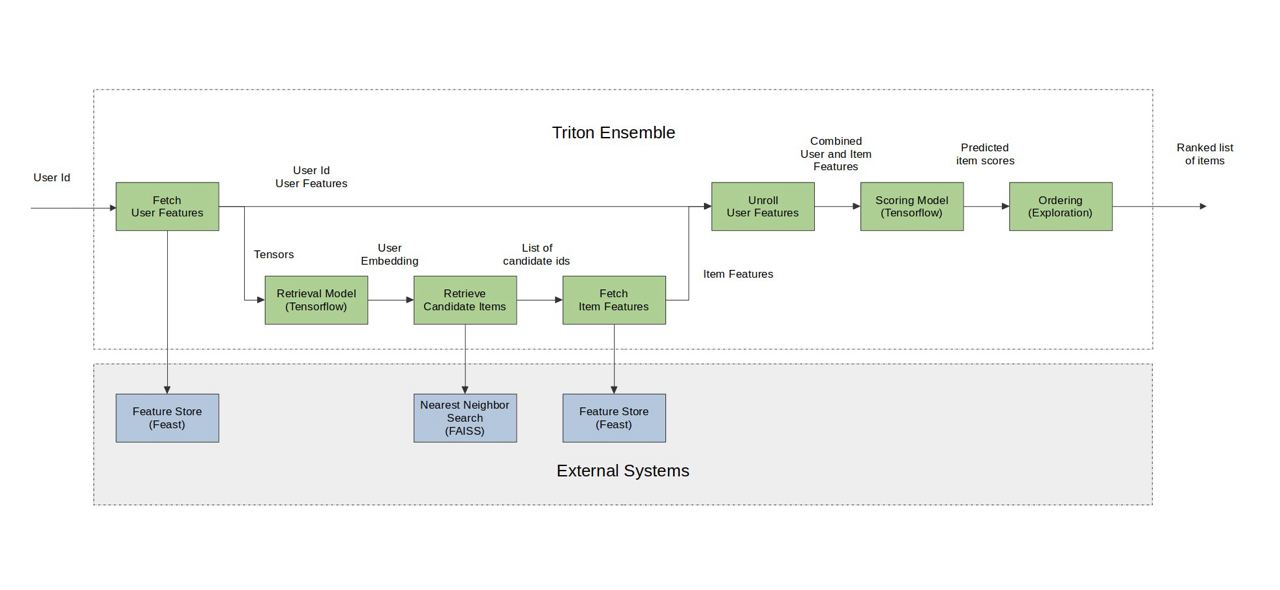
\includegraphics[width=0.8\textwidth]{assets/deployment.jpg}
    \caption{Deployment Diagram}
    \label{fig:DeploymentDiagram}
\end{figure}

The Triton Ensemble starts by fetching user features using the user ID, retrieving the necessary user-related data. These user features are then processed by a TensorFlow retrieval model to generate a user embedding. This embedding is used to retrieve a list of candidate item IDs through a nearest neighbor search. The candidate item IDs are used to fetch item features.

Next, user and item features are combined in the "Unroll User Features" step to prepare for scoring. The combined features are input into a TensorFlow scoring model, which predicts the relevance scores of each item. Finally, an ordering component uses these scores to rank the items, providing a list of recommendations.

External systems involved include a Feature Store (Feast) for storing user and item features, and FAISS for performing the nearest neighbor search. The "Fetch User Features" and "Fetch Item Features" components interact with the Feature Store to retrieve necessary data.